\chapter{Contrast Sensitivity Function Models}
\label{ch:csf}

Predicting acuity from an optical MTF requires weighting it by the human visual
system's own contrast sensitivity function (CSF) --- how sensitive the neural pathway
itself is to contrast at each spatial frequency, independent of the eye's optics. This
project uses three CSF parametrizations of deliberately different fidelity, and is
careful to always label which one produced a given number.

\section{Heuristic log-parabola models}

Two simplified, peak-location-matched log-parabola curves, normalized to $1$ at a
stated peak frequency $f_{peak}$:
\begin{equation}
\text{CSF}(f) = \exp\!\left(-\frac{(\log_2(f/f_{peak}))^2}{2\sigma^2}\right), \qquad
\sigma = \frac{\text{bandwidth (octaves)}}{2.355}
\end{equation}
with $f_{peak}=4$\,cpd (``photopic'' variant) or $f_{peak}=8$\,cpd (Mannos--Sakrison
variant). Both are explicitly documented as fit only to peak location and general
band-pass shape, \textbf{not} a full multi-parameter psychophysical model.

\section{The real Barten (1999) model}

A second, independent, luminance- and field-size-dependent CSF is used specifically
where fidelity matters most: R7acuity's neural transfer function
(Chapter~\ref{ch:r7acuity}). Its optical, neural-noise, and eye-movement terms are
\begin{align}
M_{opt}(u) &= e^{-2\pi^2\sigma^2 u^2}, & \sigma &= \sqrt{\sigma_0^2 + (C_{ab}d)^2} \\
M_{as}(u) &= \Big[ \big(X_0^{-2}+X_{max}^{-2}+u^2 N_{max}^{-2}\big)\big(Y_0^{-2}+Y_{max}^{-2}+u^2 N_{max}^{-2}\big)\Big]^{1/2} \\
S(u) &= \frac{M_{opt}(u)/k}{\sqrt{\dfrac{2}{T} M_{as}(u)\left[\dfrac{1}{npE} + \dfrac{\phi_0}{1-e^{-(u/u_0)^2}}\right]}}
\end{align}
with pupil diameter $d$ (Stanley--Davies) and retinal illuminance $E$ (with
Stiles--Crawford correction) both derived from scene luminance and field size. This
implementation is verified bit-for-bit against the published \texttt{colour-science}
open-source library's own doctested reference value
(\texttt{contrast\_sensitivity\_\allowbreak function\_\allowbreak Barten1999(4)} $=360.8691122\ldots$), which
itself cites Barten (1999, 2003) and ITU-R BT.2246-4 --- the highest-fidelity CSF used
anywhere in this project.

\begin{figure}[htbp]
\centering
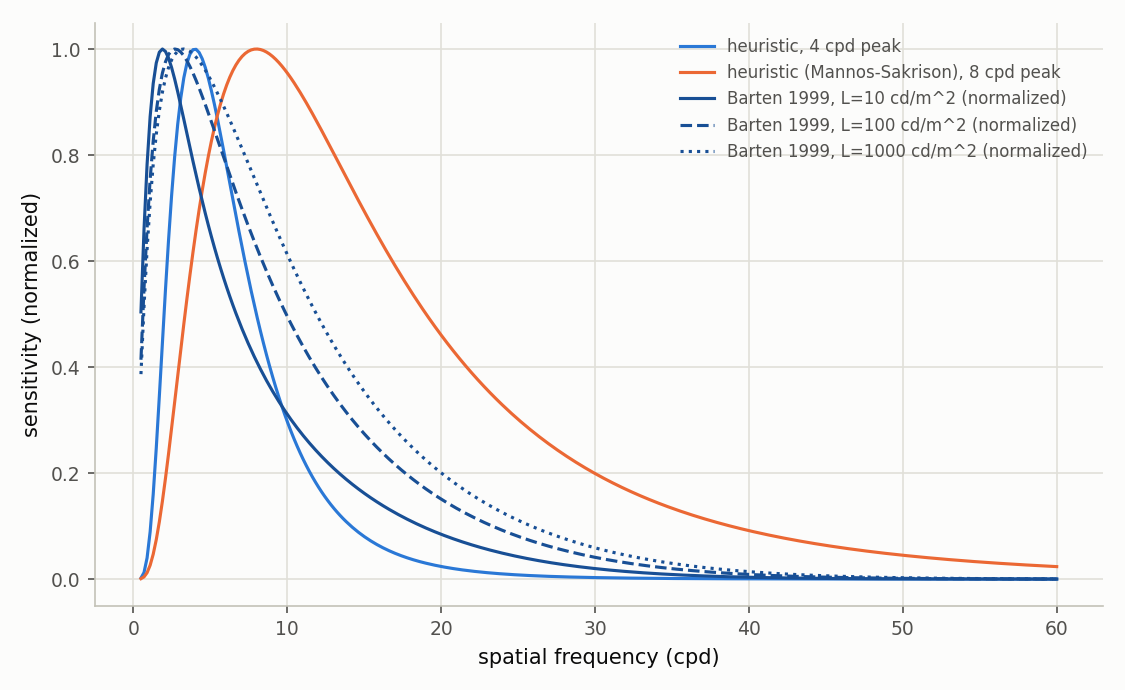
\includegraphics[width=0.85\textwidth]{figures/fig_csf_models.png}
\caption{All three CSF models: heuristic $4$\,cpd and $8$\,cpd log-parabolas, and the real Barten (1999) model at three luminance levels ($10$, $100$, $1000\,\text{cd/m}^2$).}
\label{fig:csf-models}
\end{figure}

At $L=10$, $100$, $1000\,\text{cd/m}^2$ (field diameter $20^\circ$), the real Barten
model's peak sensitivity sits at $1.90$, $2.70$, $3.30\,$cpd respectively, and cutoff
at $43.55$, $50.04$, $53.63\,$cpd --- the expected luminance-dependent CSF shift
(higher luminance sharpens and extends
sensitivity), a behavior the two heuristic models, by construction, do not reproduce
(they have no luminance argument at all).

\section{Neural transfer function}

R7acuity constructs $\text{NTF}(f) = \text{CSF}(f)/\text{MTF}_{DL}(f)$, using the
\emph{diffraction-limited} MTF (Goodman, \emph{Introduction to Fourier Optics}, 3rd
ed., \S6.3, closed form
$\text{MTF}_{DL}(f)=\frac{2}{\pi}\big[\arccos(f/f_c)-(f/f_c)\sqrt{1-(f/f_c)^2}\big]$ for
$f\le f_c$) as the denominator, not a subject's own aberrated MTF --- a deliberate
architectural choice for this project's specific two-stage design, where the real PSF
is applied separately as an optical-filtering step (Chapter~\ref{ch:r7acuity}).
